\documentclass{beamer}
\usepackage[utf8]{inputenc}
\usepackage{graphicx,wrapfig,lipsum,mdframed}
\usepackage{stmaryrd}
\usepackage{listings}
\lstset{escapeinside={<@}{@>}}
\usetheme{Warsaw}
\beamertemplatenavigationsymbolsempty
\addtobeamertemplate{navigation symbols}{}{%
	\usebeamerfont{footline}%
	\usebeamercolor[fg]{footline}%
	\hspace{1em}%
	\insertframenumber/\inserttotalframenumber
}
\setbeamertemplate{headline}{%
	\leavevmode%
	\hbox{%
		\begin{beamercolorbox}[wd=\paperwidth,ht=2.5ex,dp=1.125ex]{palette quaternary}%
			\insertsectionnavigationhorizontal{\paperwidth}{}{\hskip0pt plus1filll}
		\end{beamercolorbox}%
	}
}



\title[SQL Query evaluation with correctness guarantees]{SQL Query evaluation on Incomplete Databases with correctness guarantees}
\author[Etienne Toussaint]{Etienne Toussaint \\ supervised by Leonid Libkin}\institute{ENS Paris-Saclay, The University of Edinburgh}

\begin{document}
	
\section{Presentation}
	\begin{frame}
		\titlepage
	\end{frame}
	
	\begin{frame}
			\frametitle{University of Edinburgh, School of Informatics}
			\begin{columns}
				\begin{column}{0.48\textwidth}
					\begin{figure}
							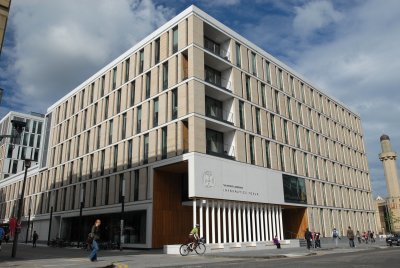
\includegraphics[scale=1.5]{forum}
							\caption{Informatics Forum}
					\end{figure}
				\end{column}
				\begin{column}{0.48\textwidth}
					\begin{itemize}
						\item Research only building
						\item 200 members
						\item 6 Institutes
					\end{itemize}
				\end{column}
			\end{columns}
			\pause
		\textbf{Laboratory for Foundations of Computer Science}
		\begin{itemize}
			\item 80 members
			\item 6 groups
		\end{itemize}
	\end{frame}
	
	\begin{frame}
		\frametitle{Database Group}
		\textbf{Database Group}
		\begin{itemize}
			\item 6 professors
			\item Weekly Seminar
		\end{itemize}
		\pause
		\bigskip
		
		\textbf{Leonid Libkin's Team}
	\begin{description}
		\item[Members] 4-7 members
		\item[Theme] Missing Information
		\item[Project] VADA: Value Added Data Systems
	\end{description}
	\end{frame}
	
	\begin{frame}
		\frametitle{SQL}
		\begin{itemize}
			\item Implemented in all major (free and commercial) RDBMSs
			\item First standardized in 1986 (ANSI) and 1987 (ISO); several revisions afterwards
			\item \$25B/year business
			\item Most common tool used by data scientists
		\end{itemize}
		\bigskip
		\begin{quote}<2>[C. Date, Database in Depth, 2005] "You can never trust the answers you get from a database with nulls". 
		\end{quote}	
		\end{frame}
		
		\section{Context}
		
		\begin{frame}
			\frametitle{Certain Answers}
			\begin{block}{Certain Answers}
				Answers independent of the interpretation of missing information
			\end{block}
			\pause
			Formally defined as :
			 $$ cert(Q, D) = \bigcap{Q(v(D))} $$
			 over all possible valuation $v$.
			 \pause
			 \begin{figure}
			 	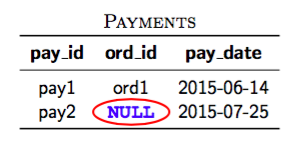
\includegraphics[scale=0.4]{pay}
			 \end{figure}
			 \begin{block}<4>{Certain Answers with nulls on bags}
			 	$$ x\in^n cert_\bot(Q,D) \iff \forall v, v(x) \in^n Q(v(D))$$
			 \end{block}
		\end{frame}
		
		\begin{frame}[containsverbatim]
			\frametitle{Answers in  SQL}
			\begin{figure}
					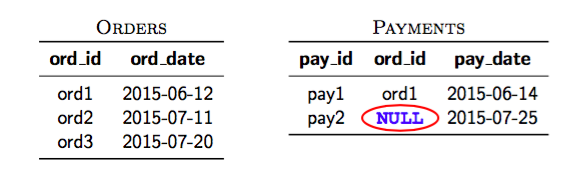
\includegraphics[scale=0.5]{db}
			\end{figure}
			A typical query to write: “Unpaid orders”
			\begin{lstlisting}[language=SQL]
SELECT ord_id FROM Orders O
WHERE NOT EXISTS  
 (SELECT * FROM Payments P 
	WHERE P.ord_id = O.ord_id)
			\end{lstlisting}
			\bigskip
		\end{frame}
		
		\begin{frame}[containsverbatim]
			\frametitle{Answers in  SQL}
			\begin{figure}
				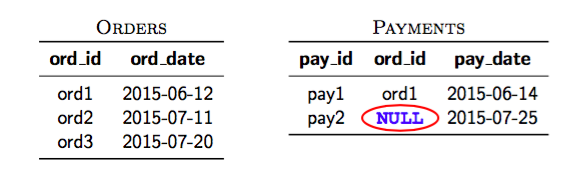
\includegraphics[scale=0.5]{db}
			\end{figure}
			A typical query to write: “Unpaid orders”
			\begin{lstlisting}[language=SQL]
SELECT ord_id FROM Orders O
WHERE NOT EXISTS  
 (SELECT * FROM Payments P 
	WHERE P.ord_id = O.ord_id)
			\end{lstlisting}
			\begin{figure}
				\textcolor{red}{Answer : $\llbracket$ord2,ord3$\rrbracket$}
			\end{figure}
		\end{frame}
		
		\begin{frame}
			\frametitle{SQL and correctness}
			\begin{block}{Correctness Guarantee}
				$$Eval(Q,D) \subseteq cert_\bot(Q,D)$$
			\end{block}
			\pause
				\textbf{SQL evaluation has NOT correctness guarantee}
			\begin{itemize}
				\item $UCQ^{\neq}$ fragment has correctness guarantee
				\item Problems arise with negative sub-queries
			
			\end{itemize}
			\pause
			\bigskip
				\textbf{Can we compute certain answers ?}
				\begin{itemize}
						\item Finding certain answers is co-NP hard
						\item SQL query answering is $AC^0$
				\end{itemize}
					\bigskip
			\pause
			\textbf{Solution: Under approximation.}
		\end{frame}
		
		\section{Algorithm}
		
		\begin{frame}
			\frametitle{The Idea}
			Translate $Q$ into   $(Q^+, Q^?)$   where:
			\begin{itemize}
				\item $Q^+$ under-approximates certain answers
				\item $Q^?$ over-approximates certain answers
			\end{itemize}
			\begin{columns}
				\begin{column}{0.52\textwidth}
					\begin{figure}
						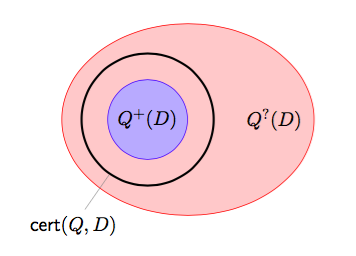
\includegraphics[scale=0.5]{slide11}
					\end{figure}
				\end{column}
				\begin{column}{0.52\textwidth}
					\begin{figure}
						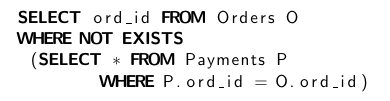
\includegraphics[scale=0.42]{q}
						\caption{$Q$}
					\end{figure}
				\end{column}
			\end{columns}
		\end{frame}
		
		\begin{frame}
			\frametitle{The translation}
			\begin{columns}
				\begin{column}{0.38\textwidth}
					\begin{figure}[h]
						\begin{mdframed}[innerleftmargin=0pt, innerrightmargin=0pt, skipabove=0pt, skipbelow=0pt, innertopmargin=0pt, innerbottommargin=0pt, nobreak=true]
							\fontsize{7}{0}
							\begin{align*}
							(H_1 \land H_2)^* & \rightarrow H_1^* \land H_2^* \\
							(H_1 \lor H_2)^* & \rightarrow H_1^* \lor H_2^* \\
							(r_i.a_i = c_i)^* & \rightarrow r_i.a_i = c_i \\
							(r_i.a_i \neq c_i)^*& \rightarrow r_i.a_i \neq c_i \\
							(r_i.a_i = r_j.a_j)^* & \rightarrow r_i.a_i = r_j.a_j \\
							(r_i.a_i \neq r_j.a_j)^* & \rightarrow r_i.a_i \neq r_j.a_j \\
							exists(Q)^* & \rightarrow exists(Q^+) \\
							notexists(Q)^* & \rightarrow notexists(Q^?) \\
							\end{align*}
						\end{mdframed}
						\caption{$Q^+$}
					\end{figure}
				\end{column}
				\begin{column}{0.6\textwidth}
					\begin{figure}[b]
						\begin{mdframed}[innerleftmargin=0pt, innerrightmargin=0pt, skipabove=0pt, skipbelow=0pt, innertopmargin=0pt, innerbottommargin=0pt, nobreak=true]
							\fontsize{7}{0}
							\begin{align*}
							(H_1 \land H_2)^{**} & \rightarrow H_1^{**} \land H_2^{**} \\
							(H_1 \lor H_2)^{**} & \rightarrow H_1^{**} \lor H_2^{**} \\
							(r_i.a_i = c_i)^{**} & \rightarrow r_i.a_i = c_i \lor null(r_i.a_i)\\
							(r_i.a_i \neq c_i)^{**}& \rightarrow r_i.a_i \neq c_i \lor null(r_i.a_i)\\
							(r_i.a_i = r_j.a_j)^{**} & \rightarrow r_i.a_i = r_j.a_j \lor null(r_i.a_i) \lor null(r_j.a_j)\\
							(r_i.a_i \neq r_j.a_j)^{**} & \rightarrow r_i.a_i \neq r_j.a_j  \lor null(r_i.a_i) \lor null(r_j.a_j)\\
							exists(Q)^{**} & \rightarrow exists(Q^?) \\
							notexists(Q)^{**} & \rightarrow notexists(Q^+) \\
							\end{align*}
						\end{mdframed}
							\caption{$Q^?$}
					\end{figure}
				\end{column}
			\end{columns}
		\end{frame}
		
		\begin{frame}
			\frametitle{Theorem}
			\begin{block}{Theorem}
				$$Q^+(D) \subseteq cert_\bot(Q,D)$$
			\end{block}
			\pause
			\begin{columns}
				\begin{column}{0.48\textwidth}
					\begin{figure}
						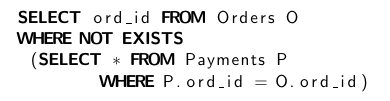
\includegraphics[scale=0.42]{q}
						\caption{$Q$}
					\end{figure}
				\end{column}
				\begin{column}{0.48\textwidth}
					\begin{figure}
						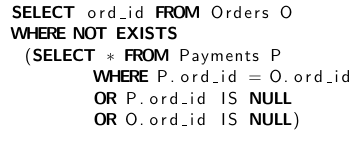
\includegraphics[scale=0.43]{rq}
						\caption{$Q^+$}
					\end{figure}
				\end{column}
			\end{columns}
			\pause
			\textbf{Evaluation of $Q^+$ is slow !}
				\begin{itemize}
					\item Quadratic vs Linear.
					\item Out of memory on big DB instances.
				\end{itemize}
				\bigskip
		\end{frame}
		
		\begin{frame}
			\frametitle{Planner}
			\begin{columns}
				\begin{column}{0.52\textwidth}
					\begin{figure}
						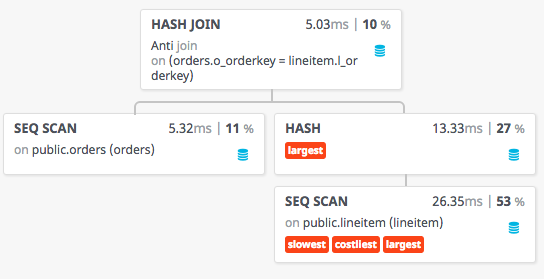
\includegraphics[scale=0.29]{qplan}
						\caption{$Q$ plan}
					\end{figure}
				\end{column}
				\begin{column}{0.52\textwidth}
					\begin{figure}
						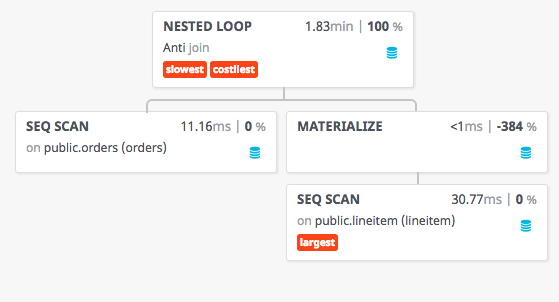
\includegraphics[scale=0.29]{rqplan}
						\caption{$Q^+$ plan}
					\end{figure}
				\end{column}
			\end{columns}
		\end{frame}
		
		
		\section{Optimisation}
		
		\begin{frame}[containsverbatim]
			\frametitle{Remove redundant Null check}
				\begin{lstlisting}[language=SQL]
SELECT ord_id FROM Orders O
 WHERE NOT EXISTS  
	(SELECT * FROM Payments P 
	 WHERE P.ord_id = O.ord_id 
	 OR <@\texttt{\textcolor{blue} {P.ord\_id IS NULL}}@>
	 OR <@\texttt{\textcolor{red}{O.ord\_id IS NULL}}@>
AND <@\texttt{\textcolor{green}{O.ord\_id = 1}}@>
OR (<@\texttt{\textcolor{blue} {P.ord\_id = 2}}@> AND <@\texttt{\textcolor{green}{O.ord\_id = 1}}@>);
				\end{lstlisting}
		\end{frame}
		
		\begin{frame}
			\frametitle{Split the query}
			\begin{columns}
				\begin{column}{0.48\textwidth}
					\begin{figure}
						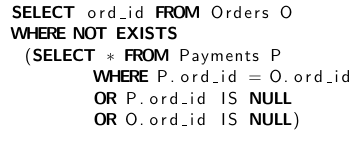
\includegraphics[scale=0.42]{rq}
						\caption{Original $Q$}
					\end{figure}
				\end{column}
				\begin{column}{0.48\textwidth}
					\begin{figure}
						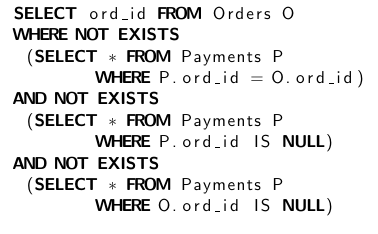
\includegraphics[scale=0.42]{rqsplit}
						\caption{Split $Q$}
					\end{figure}
				\end{column}
			\end{columns}
		\end{frame}
		
	\begin{frame}
		\frametitle{Planner}
		\begin{columns}
			\begin{column}{0.35\textwidth}
				\begin{figure}
					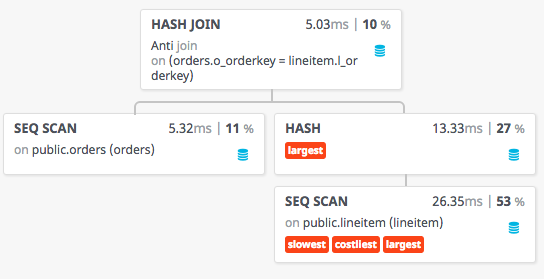
\includegraphics[scale=0.22]{qplan}
					\caption{$Q$ plan}
				\end{figure}
			\end{column}
			\begin{column}{0.60\textwidth}
				\begin{figure}
					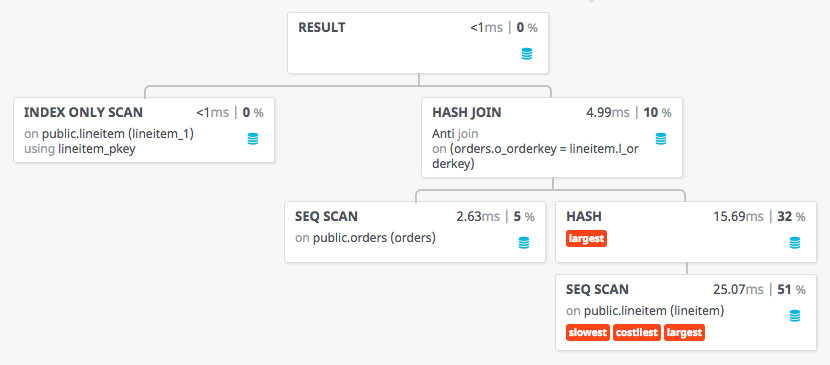
\includegraphics[scale=0.25]{orqplan}
					\caption{$Q^+$ optimize plan}
				\end{figure}
			\end{column}
		\end{columns}
	\end{frame}
		
		\section{Commentaries}
		
		\begin{frame}
			\frametitle{Implementation}
			\begin{itemize}
				\item PSQL extension (Scheme constraints)
				\item Language C
				\item Translation time insignificant (on most instances)
				\item Only a proof of concept 
				\item Fair computation time
				\item<2> Marked Nulls version
			\end{itemize}
		\end{frame}
		
		\begin{frame}
			\frametitle{Known issues}
			\begin{columns}
				\begin{column}{0.40\textwidth}
					\begin{itemize}
						\item SQL Semantic 
						\item<2->SQL Null
						\begin{itemize}
							\item<3-> Isomorphism
							\item<6-> Null multiplicity
						\end{itemize}
					\end{itemize}
				\end{column}
				\begin{column}{0.60\textwidth}
					\onslide<4->
					\begin{figure}
					\caption{Orders}
					\begin{tabular}{cc}
						\hline
						ord\_id & ord\_date \\
						\hline
						1 &  $NULL_a$ \\
						2 &  $NULL_b$ \\
						\hline
					\end{tabular}
				\end{figure}
				\onslide<5>
				\begin{figure}
					\caption{Orders $\times$ Orders}
					\begin{tabular}{cccc}
						\hline
						ord\_id & ord\_date & ord\_id & ord\_date\\
						\hline
						1 &  $NULL_a$ & 1 &  $NULL_a$\\
						2 &  $NULL_b$ & 1 &  $NULL_a$\\
						1 &  $NULL_a$ & 2 &  $NULL_b$\\
						2 &  $NULL_b$ & 2 &  $NULL_b$\\
						\hline
					\end{tabular}
				\end{figure}
				\end{column}
			\end{columns}
		\end{frame}
		
		\begin{frame}
			\frametitle{Certain answers definition}
			 \begin{block}{Certain Answers with nulls on bags}
			 	$$ x\in^n cert_\bot(Q,D) \iff \forall v, v(x) \in^n Q(v(D))$$
			 \end{block}
			 \begin{figure}
			 	\caption{Oders}
			 	\begin{tabular}{cc}
			 		\hline
			 		ord\_id & ord\_date \\
			 		\hline
			 		1 &  2015 \\
			 		2 &  2016 \\
			 		$NULL_a$ &  2016 \\
			 		\hline
			 	\end{tabular}
			 \end{figure}
			 \bigskip
			 \pause
		Wanted : \textcolor{green}{$\llbracket$1,2,$NULL_a$$\rrbracket$} \\
		\pause
		Definition : \textcolor{red}{$\llbracket$1,2,$NULL_a$,$NULL_a$$\rrbracket$}
		\end{frame}
		
		\section{Conclusion}
		
		\begin{frame}
			\frametitle{Conclusion}
			\textbf{SQL Evaluation with Correctness Guarantee}
			\begin{itemize}
				\item<1-> Theory:
					\begin{itemize}
						\item SQL semantics
						\item Certain answers with nulls definition
						\item Better approximation ?
					\end{itemize}
				\item<2-> Practice:
					\begin{itemize}
						\item Generalized Optimisation
						\item Implemented directly in DBMS
						\item Accelerate query computation ?
					\end{itemize}
			\end{itemize}
			\bigskip
			\pause
			\pause
			\textbf{SQL is only the beginning !}
		\end{frame}
\end{document}